\documentclass[journal]{IEEEtran}
\usepackage{blindtext}
\usepackage{graphicx}
\usepackage{algorithm2e}
\usepackage{amsmath}
\usepackage{amsfonts}
\usepackage{graphicx}
\usepackage{tabularx}
\usepackage{float}
\usepackage{bm}


\begin{document}

\title{GPU-Accelerated Parallelization of Edge-Based Motion Detection Algorithms with the NVIDIA CUDA Framework}

\author{
	Emilio Del Vecchio, Kevin Lin, Senthil Natarajan\\
	Department of Electrical and Computer Engineering, Rice University, Houston, TX\\
	\{edd5, kevinlin, ssn3\}@rice.edu
}

\maketitle


\begin{abstract}
Graphics processing units (GPUs) are rapidly gaining popularity as a platform for parallelized computations on massive sets of data. Since much of the computations in image processing and computer vision are easily parallelized, graphics operations on GPUs achieve significant speedups compared to those done on their serial, CPU counterparts. Further, SDKs like the NVIDIA CUDA framework provide developers easy APIs to take advantage of the parallel computing power of GPUs. In this paper, we construct a GPU-based method of real-time motion detection based on edges computed from frames of a continuous video stream, and demonstrate the speedup we can achieve compared to reference CPU implementation.
\end{abstract}


\section{Introduction}
Placeholder text

\subsection{GPU Computation}
Placeholder text

\subsection{The NVIDIA CUDA Framework}
Placeholder text


\section{Edge Detection Algorithm}
Edge detection is the process of determining the locations of boundaries that separate objects, or sections of objects, in an image. This edge data simplifies the features of an image to only its basic outlines, which makes it a convenient input for many other problems in computer vision, including motion detection and tracking, object classification, three-dimensional reconstruction, and others. The edge detection algorithm we present is composed of three stages:
\begin{enumerate}
	\item Reduce the amount of high-frequency noise from the image using a two-dimensional low pass filter.
	\item Determine the two-dimensional gradient of the filtered image by applying partial derivatives in both the horizontal and vertical directions.
	\item Classify edges by suppressing surrounding pixels in the gradient direction whose magnitude is lesser, and applying selective thresholding to a limited apron around each selected pixel.
\end{enumerate}
Edges correspond to the points on the image that exhibit a high gradient magnitude. The edge data from our algorithm is then used as input to our motion detection algorithm.

\subsection{Separable Convolution}
The filtering necessary in steps (1) and (2) from our algorithm above involve the convolution of a two-dimensional image and a two-dimensional kernel filter of constant width and height. A na\"{\i}ve implementation of two-dimensional convolution would require a double sum across the kernel and image for each individual pixel:
\begin{equation}
	\label{2d-naive-convolution}
	y[m, n] = x[m, n] * h[m, n] = \sum_{i = -\infty}^{\infty} \sum_{j = -\infty}^{\infty} h[i, j] x[m - i, n - j]
\end{equation}
For an image of size $M$ x $N$ and kernel of size $k$, a direct implementation would require $O(MNk^2)$ time, which is infeasible for a real-time implementation. Instead, it is possible to exploit the separable property of certain convolution matrices $h$, e.g. that $h$ can be represented as the product of two one-dimensional matrices $h_1$ and $h_2$. This effectively reduces our two-dimensional convolution of \eqref{2d-naive-convolution} to two separate instances of one-dimensional convolution:
$$y[m, n] = h_1[n] * (h_2[m] * x[m, n])$$
which is implemented as
$$y[m, n] = \sum_{i = -\infty}^{\infty}h_1[i] \sum_{j = -\infty}^{\infty}h_2[j] x[m - i, n - j]$$
For the same $M$ x $N$ input and square kernel of size $k$, a separable implementation reduces the computational complexity to $O(MNk)$. By comparison, an implementation using the FFT would cost $O(MN\log{MN})$. In practice, consider the following results for a convolution of a $3$ x $3$ kernel with an image of size $2500$ x $2500$:
\begin{table}[H]
	\small
	\centering
	\caption{Comparison of Computational Complexity of Different Convolution Implementation Algorithms}
	\label{convolution-complexity-comparison}
	\begin{tabular}{llll}
	 & Complexity & Execution time (s) \\
	 Direct convolution & $O(MNk^2)$ & $3$ \\
	 Separated convolution & $O(MNk)$ & $3$ \\
	 FFT & $O(MN\log{MN})$ & $3$
	\end{tabular}
\end{table}
As detailed in later sections, we take advantage of the fast computational complexity of separable convolution in our implementation, as all of the filters we apply are separable into one-dimensional matrices.


\subsection{Noise Elimination: Two-Dimensional Gaussian Filtering}
The first task in our edge detection algorithm is denoising the input in order to reduce the amount of high-frequency content in the image by as much as possible without destroying critical information points in the image (e.g. the real edges). We filter out high-frequency noise so that random noise is not mistakenly interpreted as an edge, as edges correspond to points in the image where the gradient has an above-threshold magnitude. \par
For example, consider the following $5312$ x $2988$ pixel image (taken at a high ISO to deliberately introduce noise) and a plot of its grayscale intensity versus the image's spatial dimensions:
\begin{figure}[H]
	\centering
	\includegraphics[width=0.45\textwidth]{noisy_image.jpg}
	\caption{Unfiltered noisy image}
    \label{noisy-image}
\end{figure}
\begin{figure}[h]
	\centering
	\includegraphics[width=0.45\textwidth]{noisy_image_mesh.jpg}
	\caption{Grayscale intensity of unfiltered noisy image at each pixel}
    \label{noisy-image-mesh}
\end{figure}
To low-pass filter our image, we apply a discrete Gaussian filter. Generally, a Gaussian blur kernel of size $2n + 1$ x $2n + 1$ ($\forall n \in \mathbb{Z}^+$, and with parameter $\sigma$) is given by
$$h[i, j] = \frac{1}{2\pi \sigma^2}e^{-\frac{(i - k - 1)^2 + (j - k - 1)^2}{2\sigma^2}}$$
Our implementation of Gaussian filtering uses the constant-sized ($k = 3$), constant-$\sigma$ kernel
\[
h[i, j] = \frac{1}{16}
\begin{bmatrix}
	1 & 2 & 1 \\
	2 & 4 & 2 \\
	1 & 2 & 1
\end{bmatrix}
\]
This kernel is implemented separably as
\[
h[i, j] = \frac{1}{16}
\begin{bmatrix}
	1 & 2 & 1
\end{bmatrix}
*
\begin{bmatrix}
	1 \\ 2 \\ 1
\end{bmatrix}
\] \par
Applying a Gaussian filter with parameters $k = 5$ and $\sigma = 5$ to the above image significantly denoises the image without sacrificing edge precision, which can be seen from the spatial intensity plot in Figure \ref{filtered-noisy-image-mesh}.
\begin{figure}[H]
	\centering
	\includegraphics[width=0.45\textwidth]{filtered_noisy_image.jpg}
	\caption{Gaussian-filtered noisy image with parameters $k = 3$ and $\sigma = 5$}
    \label{filtered-noisy-image}
\end{figure}
\begin{figure}[h]
	\centering
	\includegraphics[width=0.45\textwidth]{filtered_noisy_image_mesh.jpg}
	\caption{Grayscale intensity of Gaussian-filtered noisy image at each pixel}
    \label{filtered-noisy-image-mesh}
\end{figure}

\subsection{Gradient Computation: The Sobel Operator}
Edges in the image correspond to pixel locations at which there is a rapid change in intensity with respect to the image's spatial dimensions. Thus, edge pixels are defined as those whose gradient magnitude $||\boldsymbol{G}||$ is maximized along the gradient direction $\theta_G$.
\begin{equation}
	\label{gradient-magnitude}
	||\boldsymbol{G}_{i,j}|| = \sqrt{G_x^2 + G_y^2}
\end{equation}
\begin{equation}
	\label{gradient-angle}
	\theta_G = \arctan{\frac{G_y}{G_x}}
\end{equation}
where $G_x$ and $G_y$ are the values of the partial derivatives along the $x$ and $y$ directions, respectively, at the pixel located at $(i, j)$ of the image $A$.
$$G_x = \frac{\partial \boldsymbol{A}}{\partial x}\Bigr|_{\substack{(x, y) = (i, j)}}$$
$$G_y = \frac{\partial \boldsymbol{A}}{\partial y}\Bigr|_{\substack{(x, y) = (i, j)}}$$
\par A variety of different discrete differentiation operators exist to approximate the gradient of the image. The operator we choose in our implementation is the Sobel operator.
\[
\boldsymbol{G_x} =
\begin{bmatrix}
	-1 & 0 & 1 \\
	-2 & 0 & 2 \\
	-1 & 0 & 1
\end{bmatrix} * \boldsymbol{A}
\]
\[
\boldsymbol{G_y} =
\begin{bmatrix}
	-1 & -2 & -1 \\
	0 & 0 & 0 \\
	1 & 2 & 1
\end{bmatrix} * \boldsymbol{A}
\]
Like our Gaussian kernel, the Sobel operator (in both the $x$ and $y$ directions) is separable:
\[
\boldsymbol{G_x} =
\begin{bmatrix}
	1 \\
	2 \\
	1
\end{bmatrix} * 
(\begin{bmatrix}
	1 & 0 & -1
\end{bmatrix} * \boldsymbol{A})
\]
\[
\boldsymbol{G_y} =
\begin{bmatrix}
	1 \\
	0 \\
	-1
\end{bmatrix} * 
(\begin{bmatrix}
	1 & 2 & 1
\end{bmatrix} * \boldsymbol{A})
\]
\par Thus, we perform two separable convolutions with the separated Sobel filter on the Gaussian-filtered image to obtain gradients in the horizontal and vertical directions, and determine the magnitude and angle matrices $\boldsymbol{G}$ and $\boldsymbol{\theta}$ from equations \eqref{gradient-magnitude} and \eqref{gradient-angle}.
\begin{figure}[h]
	\centering
	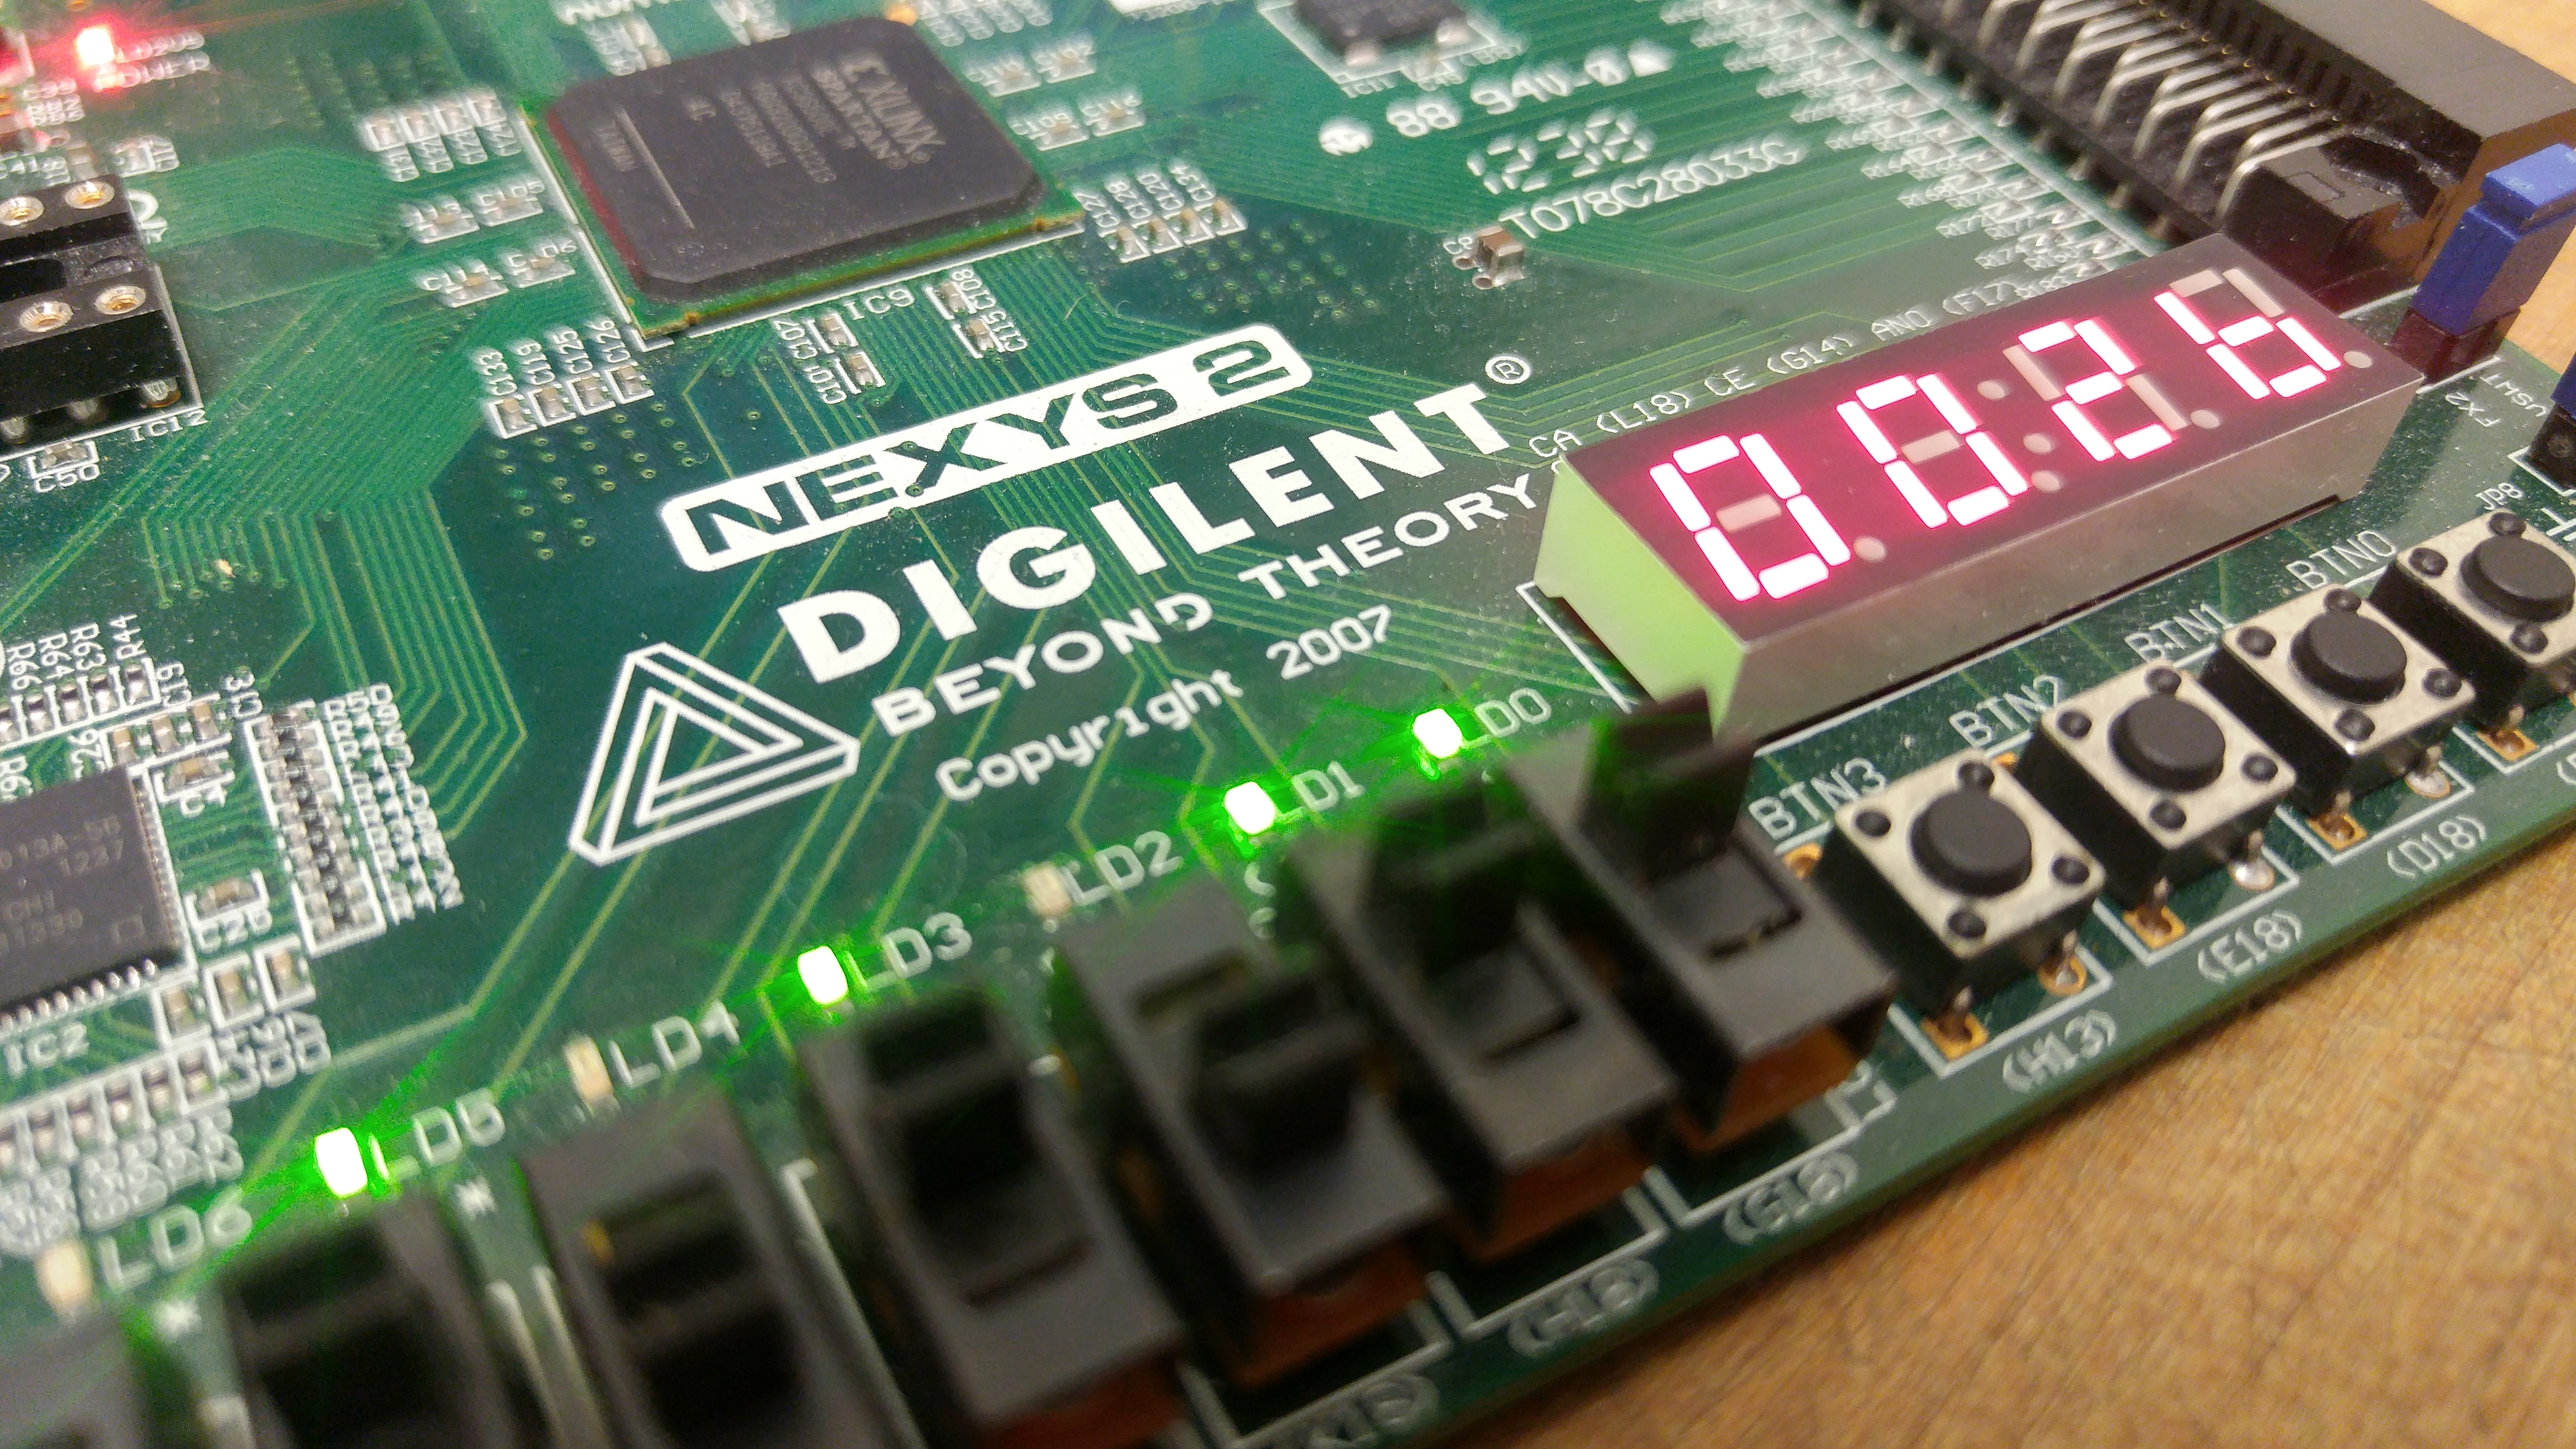
\includegraphics[width=0.45\textwidth]{pcb.jpg}
	\caption{Original image input to Sobel filter}
    \label{pcb-original}
\end{figure}
\begin{figure}[h]
	\centering
	\includegraphics[width=0.45\textwidth]{sobel_pcb.jpg}
	\caption{Magnitude of the gradient $||\boldsymbol{G}||$, as determined by applying a Sobel filter in both the $x$ and $y$ directions, at each pixel of the Gaussian-filtered original image with parameters $k = 5$ and $\sigma = 5$}
    \label{sobel-pcb}
\end{figure}
\begin{figure}[h]
	\centering
	\includegraphics[width=0.45\textwidth]{sobel_pcb_mesh.jpg}
	\caption{Gradient of \ref{sobel-pcb} visualized as a three-dimensional mesh}
    \label{sobel-pcb}
\end{figure}

\subsection{Non-Maximum Suppression and Selective Thresholding}
Given the gradient magnitude and direction of the Gaussian-filtered image, the final step of the edge detection algorithm is to determine which pixels should be selected as edge pixels, and which should be rejected. We define two procedures, \textit{non-maximum suppression} and \textit{selective thresholding}, to gain a reasonably accurate edge map from the gradient.
\par Non-maximum suppression selects and rejects edge pixels according to the following criteria:
\begin{enumerate}
	\item Pixels whose gradient magnitude is below a user-defined low threshold, $t_l$, is immediately rejected
	\item If the gradient magnitude of a pixel is greater than that of the pixels in either direction of the gradient angle of that pixel, then the pixel is accepted if its gradient magnitude is greater than a user-defined high threshold, $t_h$
\end{enumerate}
More precisely, a pixel at $(i, j)$ with gradient magnitude $G_{i, j} > t_l$ and angle $\theta$ is accepted if any of the following hold true:
\begin{itemize}
	\item $(-\frac{\pi}{6} < \theta < \frac{\pi}{6} \vee -\pi < \theta < -\frac{5 \pi}{6} \vee \frac{5\pi}{6} < \theta < \pi) \wedge G_{i, j} > G_{i, j \pm 1}$
	\item $(\frac{\pi}{6} < \theta < \frac{\pi}{3} \vee -\frac{5 \pi}{6} < \theta < -\frac{2 \pi}{3}) \wedge G_{i, j} > G_{i \pm 1, \pm j}$
	\item $(\frac{\pi}{3} < \theta < \frac{2 \pi}{3} \vee -\frac{2 \pi}{3} < \theta < -\frac{\pi}{3}) \wedge G_{i, j} > G_{i \pm 1, j}$
	\item $(\frac{2 \pi}{3} < \theta < \frac{5 \pi}{6} \vee -\frac{\pi}{3} < \theta < -\frac{\pi}{6}) \wedge G_{i, j} > G_{i \pm 1, \mp j}$
\end{itemize}
The selective thresholding technique extends on the procedure of non-maximum suppression. For any pixel that passes crtiteria (2) (maximized, relative to the neighboring pixels, along the gradient direction), consider an $\alpha$ x $\alpha$ box around the pixel. If any pixel within the box exceeds the low threshold $t_l$, then the pixel is accepted. This technique attempts to catch pixels that might ``connect" ridge pixels identified by criteria (2) but fail to satify the criterion themselves, in order to create more continuous edge lines.


\section{Motion Detection Algorithm}
Placeholder text

\subsection{Thresholded Frame-by-Frame Difference Map}
Placeholder text

\subsection{Motion Area Estimation via a Spatial Difference Density Map}
Placeholder text


\section{GPU Speedup Results}
Placeholder text


\section{Conclusion}
Placeholder text

\appendices
\section{Proof of the First Zonklar Equation}
Some text for the appendix.

\section*{Acknowledgment}
\begin{thebibliography}{1}

\bibitem{IEEEhowto:kopka}
H.~Kopka and P.~W. Daly, \emph{A Guide to \LaTeX}, 3rd~ed.\hskip 1em plus
  0.5em minus 0.4em\relax Harlow, England: Addison-Wesley, 1999.

\end{thebibliography}
\end{document}